\chapter{शरीर-योजनाएँ और साझा पूर्वज}\label{ch:g10:common-ancestry}

अपनी बाँह फैलाइए और गिनिए: कंधे से कोहनी तक एक हड्डी, कोहनी से कलाई तक
दो, कलाई में छोटी हड्डियों का एक गुच्छा, और पाँच उँगलियाँ। अब चमगादड़ के
पंख, ह्वेल के फ़्लिपर, घोड़े की अगली टाँग और मेंढक की बाँह का कंकाल
देखिए: वही एक हड्डी, दो हड्डियाँ, गुच्छा और अंगुलियाँ --- कहीं खिंची,
कहीं जुड़ी, कहीं छोटी, पर उनका क्रम कभी नहीं बदला। शून्य से कोई पंख
डिज़ाइन करने वाला किसी बाँह से शुरू नहीं करता। यह मिलाप किसी विरासत में
मिली चीज़ का निशान है, और यह अध्याय ऐसे ही निशान पढ़ने के बारे में है ---
कंकालों में, भ्रूणों में, अणुओं में --- ताकि सजीवों की नातेदारी दोबारा
खड़ी की जा सके।

\section{कशेरुकियों की शरीर-योजना}

\begin{definition}[शरीर-योजना]\label{def:g10:common-ancestry:bodyplan}
जीवों के किसी समूह की \emph{शरीर-योजना}\index{शरीर-योजना} उनके हिस्सों का
वह साझा विन्यास है: सममिति के अक्ष और मुख्य अंगों की सापेक्ष स्थितियाँ,
चाहे आकार, रूप या जीने का ढंग कुछ भी हो। \emph{कशेरुकी}\index{कशेरुकी}
--- मछलियाँ, उभयचर, सरीसृप, पक्षी, स्तनधारी --- एक ही योजना बाँटते हैं:
एक ऊर्ध्वाधर तल के इर्द-गिर्द सममित शरीर, जिसका अगला सिरा सिर ढोता है और
जिसका एक पिछला सिरा है; एक भीतरी कंकाल, जिसका अक्ष कशेरुकों का एक दंड है
और जो पृष्ठीय तंत्रिका रज्जु की रक्षा करता है; और पाचन नली, जो अधर की ओर
चलती है, मुँह आगे रहता है, और हृदय उसके नीचे।
\end{definition}

\begin{omfigure}
\begin{tikzpicture}[font=\small, >=Stealth]
  % generic vertebrate side view
  \draw[thick, fill=omDef!6, rounded corners=14pt] (0,0) rectangle (9,3.2);
  \draw[thick, omThm] (0.6,2.5) -- (8.6,2.5);                      % nerve cord
  \foreach \x in {1.2,1.8,...,8.4} \draw[thick] (\x,2.15) -- (\x,2.35); % vertebrae
  \draw[thick] (1.0,2.25) -- (8.6,2.25);
  \draw[thick, omProp, fill=omProp!20] (0.5,1.4) .. controls (2,0.7) and (6,0.7) .. (8.6,1.2)
    .. controls (6,1.5) and (2,1.9) .. (0.5,1.4);                      % gut
  \draw[thick, omThm, fill=omThm!30] (2.3,0.75) circle (0.32);         % heart
  \node[anchor=west] at (9.4,2.5) {तंत्रिका रज्जु (पृष्ठीय)};
  \draw[->] (9.35,2.5) -- (8.65,2.5);
  \node[anchor=west] at (9.4,2.0) {कशेरुक दंड};
  \draw[->] (9.35,2.0) -- (8.6,2.22);
  \node[anchor=west] at (9.4,1.2) {पाचन नली (अधर)};
  \draw[->] (9.35,1.2) -- (8.65,1.2);
  \node[anchor=north] at (2.3,-0.1) {हृदय, नली के नीचे};
  \draw[->] (2.3,-0.05) -- (2.3,0.4);
  \node[anchor=east] at (-0.1,1.4) {मुँह};
  \draw[->] (-0.05,1.4) -- (0.45,1.4);
  \node[anchor=south, font=\small\itshape] at (4.5,3.3) {पृष्ठीय ओर};
  \node[anchor=north, font=\small\itshape] at (6.5,-0.05) {अधर ओर};
  \draw[<->, gray] (0,3.7) -- (9,3.7) node[midway, above, font=\scriptsize] {आगे--पीछे का अक्ष};
\end{tikzpicture}

{\small \omterm{def:g10:common-ancestry:bodyplan}{कशेरुकियों} की \omterm{def:g10:common-ancestry:bodyplan}{शरीर-योजना}, बग़ल से। \omterm{def:g10:biodiversity-scales:species}{जाति} कोई भी हो, तंत्रिका
रज्जु पीठ के साथ-साथ कशेरुक दंड के ऊपर चलती है, पाचन नली पेट के साथ-साथ,
और हृदय उसके नीचे आगे की ओर। कीटों और केंचुओं में तंत्रिका रज्जु अधर की
ओर होती है: यानी एक अलग योजना।}
\end{omfigure}

\begin{example}[एक ही योजना, अलग-अलग जंतु]\label{ex:g10:common-ancestry:sameplan}
ट्राउट, मेंढक, छिपकली, कबूतर और चूहे को अग़ल-बग़ल चीरकर देखा जाए तो हर
हाल में वही योजना दिखती है: पीठ में मेरुरज्जु, जिसकी रक्षा कशेरुक करते
हैं; उसके नीचे आँत, और आमाशय के बग़ल में यकृत; आगे की ओर, आँत के नीचे
हृदय; और हड्डी की मेखलाओं से जुड़े जोड़ेदार उपांग (या पख)। जो फ़र्क़ हैं
--- क्लोम या फेफड़े, पख या टाँगें, शल्क, पंख या रोएँ --- वे सब उसी एक
विन्यास पर खड़े रूपभेद हैं।
\end{example}

\section{समजात अंग}

\begin{definition}[समजातता]\label{def:g10:common-ancestry:homology}
दो \omterm{def:g10:biodiversity-scales:species}{जातियों} के दो अंग \emph{समजात}\index{समजातता} तब होते हैं जब उनकी
बनावट और \omterm{def:g10:common-ancestry:bodyplan}{शरीर-योजना} में उनकी स्थिति एक ही हो --- यानी वे उन्हीं हिस्सों
से उन्हीं संबंधों में बने हों --- चाहे आज उनका काम कुछ भी हो। चतुष्पादों
के अगले उपांग इसका मानक उदाहरण हैं: एक हड्डी (ह्यूमरस), दो हड्डियाँ
(रेडियस और अल्ना), कलाई की हड्डियों का एक गुच्छा, और फिर अंगुलियाँ। जो
अंग एक ही काम अलग बनावट से करते हैं --- किसी पक्षी का पंख और किसी मक्खी
का पंख --- वे केवल \emph{समवृत्ति} हैं, और नातेदारी के बारे में कुछ नहीं
कहते।
\end{definition}

\begin{omfigure}
\begin{tikzpicture}[font=\small, line cap=round]
  % three stylised forelimbs: humerus (red), radius+ulna (blue), carpals (gray), digits (green)
  \tikzset{hum/.style={line width=6pt, omThm!70},
           ru/.style={line width=4pt, omDef!70},
           carp/.style={fill=gray!50, draw=gray!70},
           dig/.style={line width=3pt, omMeth!80}}
  % human arm
  \begin{scope}
    \draw[hum] (0,3.2) -- (0.2,1.9);
    \draw[ru] (0.1,1.85) -- (0.3,0.9); \draw[ru] (0.35,1.85) -- (0.5,0.9);
    \fill[carp] (0.15,0.7) rectangle (0.65,0.85);
    \foreach \dx in {-0.3,-0.12,0.05,0.22,0.4} \draw[dig] (0.4,0.7) -- ({0.4+\dx},-0.1);
    \node[anchor=north] at (0.4,-1.4) {मनुष्य की बाँह};
  \end{scope}
  % bat wing
  \begin{scope}[xshift=3.6cm]
    \draw[hum] (0,3.2) -- (0.4,2.3);
    \draw[ru] (0.4,2.3) -- (1.0,1.3);
    \fill[carp] (0.95,1.2) rectangle (1.25,1.35);
    \draw[dig] (1.1,1.2) -- (0.8,0.9);
    \foreach \a in {-0.6,-0.3,0.1,0.5} \draw[dig] (1.1,1.2) -- ({1.1+2.2*cos(-60+40*\a)},{1.2+2.2*sin(-60+40*\a)});
    \node[anchor=north] at (1.2,-1.4) {चमगादड़ का पंख};
  \end{scope}
  % whale flipper
  \begin{scope}[xshift=8.0cm]
    \draw[hum] (0,3.2) -- (0.1,2.5);
    \draw[ru] (0.0,2.45) -- (0.05,1.9); \draw[ru] (0.3,2.45) -- (0.35,1.9);
    \fill[carp] (-0.05,1.6) rectangle (0.5,1.85);
    \foreach \dx in {-0.2,0.0,0.2,0.45} \draw[dig] ({0.22+0.5*\dx},1.6) -- ({0.22+\dx},0.2);
    \draw[gray!60, rounded corners=8pt] (-0.5,3.4) -- (-0.6,0.0) -- (0.9,-0.1) -- (0.9,3.4);
    \node[anchor=north] at (0.2,-1.4) {ह्वेल का फ़्लिपर};
  \end{scope}
  % legend
  \begin{scope}[xshift=10.4cm, yshift=2.2cm]
    \draw[hum] (0,1.0) -- (0.6,1.0); \node[anchor=west] at (0.7,1.0) {ह्यूमरस};
    \draw[ru] (0,0.5) -- (0.6,0.5); \node[anchor=west] at (0.7,0.5) {रेडियस, अल्ना};
    \fill[carp] (0.05,-0.08) rectangle (0.55,0.08); \node[anchor=west] at (0.7,0) {कलाई की हड्डियाँ};
    \draw[dig] (0,-0.5) -- (0.6,-0.5); \node[anchor=west] at (0.7,-0.5) {अंगुलियाँ};
  \end{scope}
\end{tikzpicture}

{\small तीन \omterm{def:g10:common-ancestry:homology}{समजात} अगले उपांग, आरेख के रूप में: वही हड्डियाँ उसी क्रम में,
कहीं खिंचकर पंख, कहीं चपटी होकर फ़्लिपर। काम अलग है; बनावट और स्थिति
नहीं।}
\end{omfigure}

\begin{omfigure}
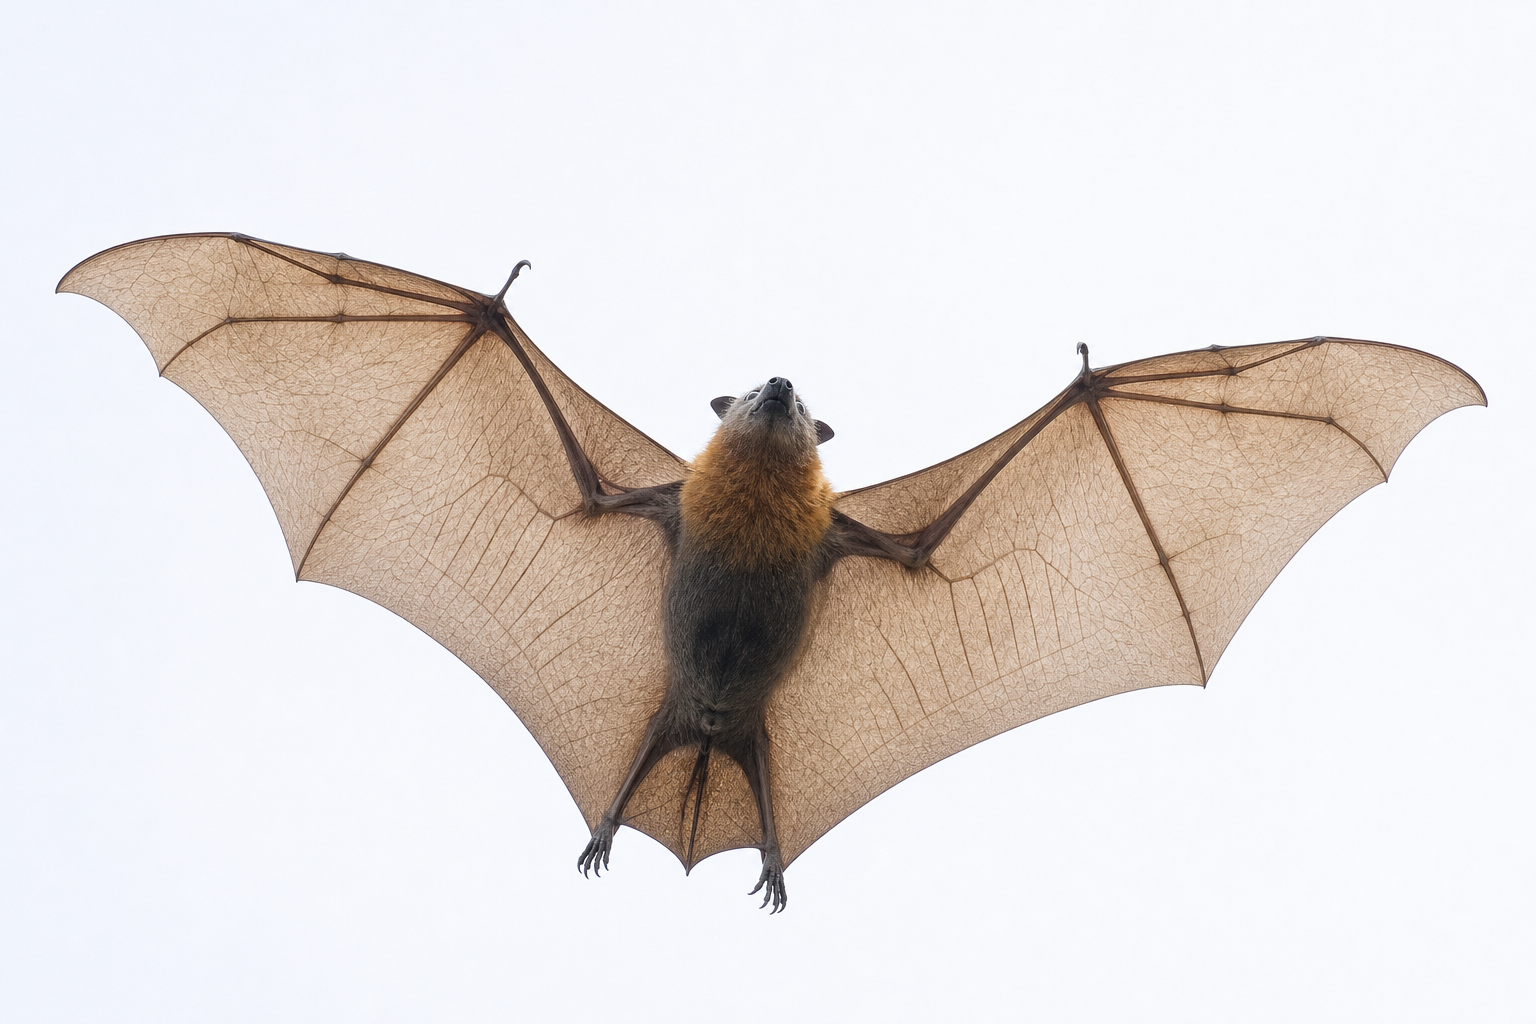
\includegraphics[width=0.6\linewidth]{images/book2/ai/g10-ancestry-bat-wing.png}

{\small उड़ान भरता एक चमगादड़: पंख की झिल्ली बेहद लंबी हो चुकी उँगलियों की
हड्डियों पर तनी है। स्तनधारी योजना का हाथ, पंख में बदला हुआ।}
\end{omfigure}

\begin{proposition}[समजातता नातेदारी खोलती है]\label{prop:g10:common-ancestry:kinship}
साझा \omterm{def:g10:common-ancestry:homology}{समजात} रचनाएँ किसी ऐसे साझा पूर्वज से विरासत में मिली हैं जिसके पास
वे थीं; और दो \omterm{def:g10:biodiversity-scales:species}{जातियाँ} जितनी अधिक ऐसी रचनाएँ बाँटती हैं, उनकी नातेदारी
उतनी ही क़रीब की है। चतुष्पाद उपांग हर थलचर \omterm{def:g10:common-ancestry:bodyplan}{कशेरुकी} में मिलता है, क्योंकि
सब उसी एक पूर्वज वंशक्रम से उतरे हैं जिसके पास वह था; और चमगादड़ का पंख
एक बदली हुई बाँह है, क्योंकि चमगादड़ बाँहों वाले स्तनधारियों से उतरे हैं,
पक्षियों से नहीं।
\end{proposition}
\begin{proof}[साक्ष्य]
तीन स्वतंत्र दिशाएँ एक जगह मिलती हैं। \emph{जीवाश्म}: तिथि लगी चट्टानों
के क्रम में ऐसे रूप मिलते हैं जिनमें अभिलक्षणों के बीच के मेल हैं ---
37.5 करोड़ साल पहले उपांग जैसे पखों और गरदन वाली मछलियाँ, और फिर मछली
जैसी पूँछ वाले चौपाए; तथा 15 करोड़ साल पुराना \emph{Archaeopteryx},
जिसके पंख और डैने तो हैं ही, दाँत, पंजेदार उँगलियाँ और एक लंबी हड्डीदार
पूँछ भी। \emph{भ्रूण}: \omterm{def:g10:common-ancestry:bodyplan}{कशेरुकियों} के सारे भ्रूण एक ऐसी अवस्था से गुज़रते
हैं जिसमें क्लोम-थैलियाँ, एक पूँछ और एक पृष्ठरज्जु होती है --- वे रचनाएँ
जो वयस्क मछली में बनी रहती हैं और बाक़ियों में बदल दी जाती हैं या खो जाती
हैं। \emph{अणु}: जैसा \cref{ch:g10:universal-dna} ने दिखाया, सबके पास \omterm{def:g10:universal-dna:information}{DNA}
और वही \omterm{def:g10:universal-dna:gene}{जीन} हैं, और किसी एक \omterm{def:g10:universal-dna:gene}{जीन} के रूपों के बीच के फ़र्क़ \omterm{def:g10:biodiversity-scales:species}{जातियों} को
ठीक वैसे ही क्रम में रखते हैं जैसे शरीर-रचना रखती है।
\end{proof}

\begin{omfigure}
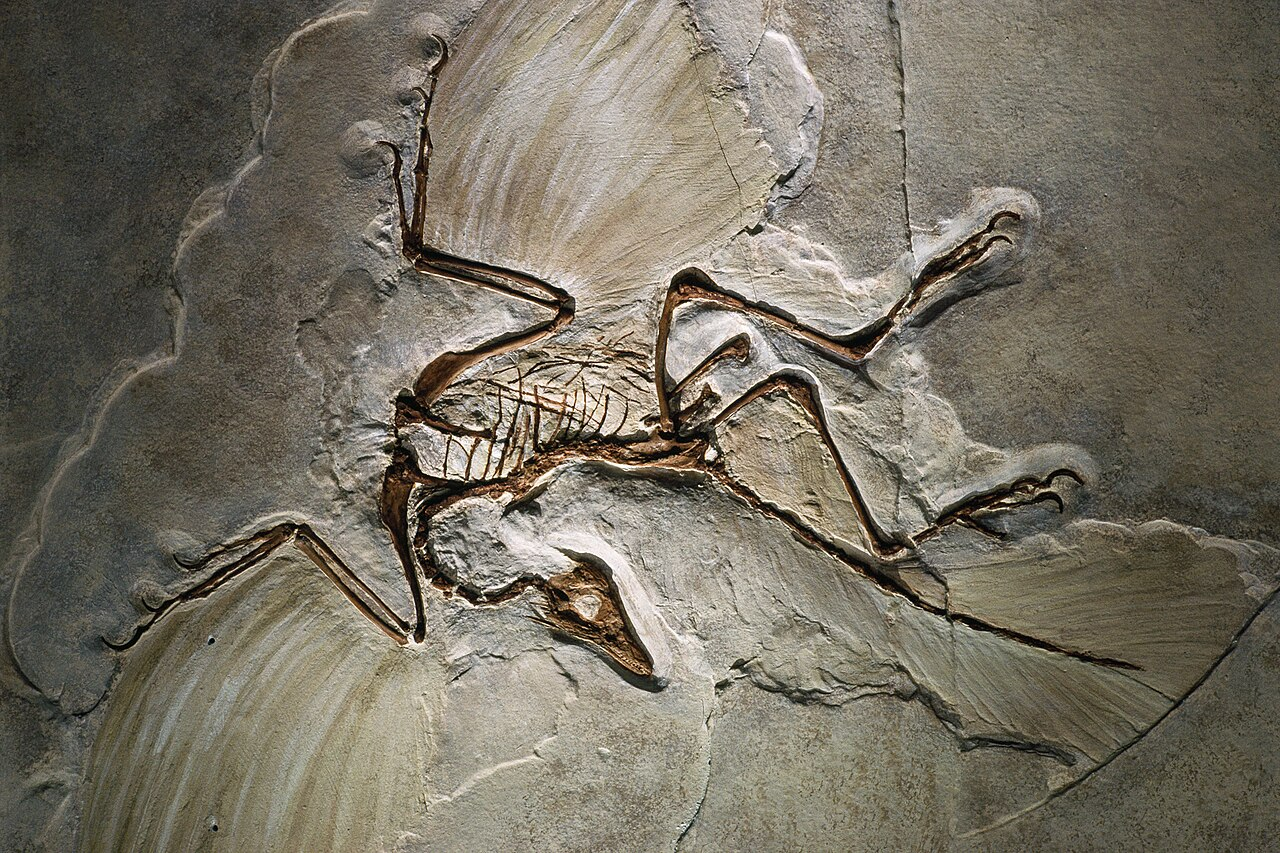
\includegraphics[width=0.5\linewidth]{images/book1/archaeopteryx.jpg}

{\small \emph{Archaeopteryx}, 15 करोड़ साल पुराना: पक्षी जैसे परदार डैने
और द्विशाखी हड्डी, और साथ में दाँत, पंजेदार उँगलियाँ तथा किसी छोटे
डायनासोर जैसी लंबी हड्डीदार पूँछ। दो समूहों के अभिलक्षण मिलाता जीवाश्म
ठीक वही है जिसकी भविष्यवाणी साझा पूर्वज करते हैं। फ़ोटो जेम्स एल॰ एमोस,
CC0।}
\end{omfigure}

\section{एक-दूसरे में धँसे समूह}

\begin{method}[साझा अभिलक्षणों से समूह बनाना]\label{met:g10:common-ancestry:grouping}
नातेदारी के समूह साझा \emph{व्युत्पन्न} अभिलक्षणों से बनाए जाते हैं ---
यानी उन गुणों से जो किसी पूर्वज में एक बार उभरे और उसके सारे वंशजों को
विरासत में मिले।
\begin{enumerate}
  \item \omterm{def:g10:biodiversity-scales:species}{जातियाँ} और अभिलक्षणों का एक समुच्चय गिनाइए (कशेरुक दंड; चार
        उपांग; खोल वाला अंडा या उसका समकक्ष, यानी उल्बयुक्त अंडा; परों
        वाले डैने; रोएँ और दूध; और इसी तरह)।
  \item हर अभिलक्षण के लिए नोट कीजिए कि वह किन \omterm{def:g10:biodiversity-scales:species}{जातियों} के पास है।
  \item किसी उपसमुच्चय का साझा अभिलक्षण एक समूह तय करता है: चार उपांगों
        वाली सारी \omterm{def:g10:biodiversity-scales:species}{जातियाँ} चतुष्पाद हैं; उनमें से उल्बयुक्त अंडे वाली
        सब उल्बधारी; और उनमें से रोएँ वाली सब स्तनधारी।
  \item समूहों को एक-दूसरे में धँसे डिब्बों के रूप में खींचिए, या ऐसे
        वृक्ष के रूप में जिसकी हर गाँठ वह साझा पूर्वज हो जिसमें वह
        अभिलक्षण उभरा। किसी समूह में उस पूर्वज के \emph{सारे} वंशज होने
        चाहिए: रोज़मर्रा के अर्थ वाली ``मछलियाँ'' या ``सरीसृप'' ऐसे समूह
        नहीं हैं।
\end{enumerate}
\end{method}

\begin{omfigure}
\begin{tikzpicture}[font=\small]
  \node[draw, rounded corners, thick, fill=omDef!6, minimum width=12.2cm, minimum height=4.6cm] (v) at (0,0) {};
  \node[anchor=north west] at (v.north west) {\ \textbf{कशेरुकी}: कशेरुक दंड};
  \node[anchor=south west] at (v.south west) {\ ट्राउट};
  \node[draw, rounded corners, thick, fill=omMeth!8, minimum width=9.6cm, minimum height=3.5cm] (t) at (0.9,-0.25) {};
  \node[anchor=north west] at (t.north west) {\ \textbf{चतुष्पाद}: चार उपांग};
  \node[anchor=south west] at (t.south west) {\ मेंढक};
  \node[draw, rounded corners, thick, fill=omProp!10, minimum width=7.0cm, minimum height=2.4cm] (a) at (1.8,-0.5) {};
  \node[anchor=north west] at (a.north west) {\ \textbf{उल्बधारी}: उल्बयुक्त अंडा};
  \node[anchor=south west] at (a.south west) {\ छिपकली\quad कबूतर};
  \node[draw, rounded corners, thick, fill=omThm!10, minimum width=3.7cm, minimum height=1.3cm] (m) at (3.2,-0.75) {};
  \node[anchor=north west] at (m.north west) {\ \textbf{स्तनधारी}: रोएँ, दूध};
  \node[anchor=south west] at (m.south west) {\ चूहा\quad मनुष्य};
\end{tikzpicture}

{\small पाँच \omterm{def:g10:common-ancestry:bodyplan}{कशेरुकियों} के एक-दूसरे में धँसे नातेदारी-समूह। हर डिब्बा उस
अभिलक्षण से तय होता है जो उसके भीतर की हर चीज़ के साझा पूर्वज में एक बार
उभरा था। कबूतर छिपकली के साथ ``उल्बधारी'' के भीतर है: यानी छिपकली मेंढक
के मुक़ाबले कबूतर की अधिक क़रीबी नातेदार है।}
\end{omfigure}

\begin{example}[डिब्बे पढ़ना]\label{ex:g10:common-ancestry:reading}
ट्राउट, मेंढक, छिपकली और कबूतर में से चूहे का सबसे क़रीबी नातेदार कौन है?
चूहे और किसी दूसरी \omterm{def:g10:biodiversity-scales:species}{जाति} को साथ रखने वाला सबसे छोटा डिब्बा
``उल्बधारी'' है, जिसमें छिपकली और कबूतर हैं: वे दोनों बराबर क़रीबी हैं,
दोनों चूहे के मेंढक से अधिक क़रीब, और मेंढक ट्राउट से अधिक क़रीब। छिपकली
मेंढक के बजाय कबूतर के क़रीब हो, यह अधिकांश लोगों को चौंकाता है; पर खोल
वाला अंडा, जो किसी मेंढक के पास नहीं, इसे तय कर देता है।
\end{example}

\section{अणुओं में नातेदारी}

\begin{proposition}[आणविक नातेदारी]\label{prop:g10:common-ancestry:molecular}
चूँकि सारे सजीव साझा पूर्वजों से उतरे हैं, इसलिए दो \omterm{def:g10:biodiversity-scales:species}{जातियों} में मौजूद
कोई \omterm{def:g10:universal-dna:gene}{जीन} उसी पूर्वज \omterm{def:g10:universal-dna:gene}{जीन} की बदली हुई प्रति है, और दोनों प्रतियों के बीच
फ़र्क़ों की संख्या उन \omterm{def:g10:biodiversity-scales:species}{जातियों} के अलग होने के बाद बीते समय के साथ बढ़ती
है। इसलिए किसी एक \omterm{def:g10:universal-dna:gene}{जीन} का, या उसके कूट वाले \omterm{def:g10:chemistry-of-life:families}{प्रोटीन} का, अनुक्रम अलग-अलग
\omterm{def:g10:biodiversity-scales:species}{जातियों} में मिलाकर देखना नातेदारी नापता है, और जो समूह इससे बनते हैं वे
शरीर-रचना से बने समूहों से मेल खाते हैं।
\end{proposition}
\admitted

\begin{example}[साइटोक्रोम c]\label{ex:g10:common-ancestry:cytochrome}
साइटोक्रोम c लगभग 104 \omterm{def:g10:chemistry-of-life:families}{ऐमीनो अम्लों} का एक \omterm{def:g10:chemistry-of-life:families}{प्रोटीन} है, जिसे हर सुकेंद्रकी
जीव श्वसन में इस्तेमाल करता है। मनुष्य के अनुक्रम से मिलाने पर
चिंपैंज़ी का 0 स्थानों पर अलग है, चूहे का 9 पर, मुर्ग़ी का 13 पर, मेंढक
का 18 पर, टूना का 21 पर, और खमीर का 45 पर। फ़र्क़ों के हिसाब से क्रम में
रखें तो \omterm{def:g10:biodiversity-scales:species}{जातियाँ} ठीक पिछले चित्र के डिब्बों में गिरती हैं: पहले
स्तनधारी, फिर उल्बधारी, फिर चतुष्पाद, फिर \omterm{def:g10:common-ancestry:bodyplan}{कशेरुकी}, फिर सुकेंद्रकी।
\end{example}

\begin{remark}[एकता और नातेदारी]\label{rem:g10:common-ancestry:unity}
संघटन की एकता (\cref{ch:g10:chemistry-of-life}), \omterm{def:g10:cells-common-unit:cell}{कोशिका} की एकता
(\cref{ch:g10:cells-common-unit}), आनुवंशिक अणु की एकता
(\cref{ch:g10:universal-dna}) और अब शरीर-योजनाओं तथा जीन-अनुक्रमों की
एकता --- ये एक ही तथ्य के चार दर्शन हैं: सजीव इसलिए एक-दूसरे से
मिलते-जुलते हैं कि वे नातेदार हैं, और वे इसलिए नातेदार हैं कि वे साझा
पूर्वजों से उतरे हैं। \cref{ch:g10:biodiversity-scales} की विविधता उसी
वंशक्रम में रूपांतरण के साथ उतरने का नतीजा है, उस समय के दौरान जिसे
जीवाश्मों का लेखा नापता है। ये रूपांतरण उभरते और फैलते कैसे हैं, यह
आख़िरी वर्ष का विषय है।
\end{remark}

\section{अभ्यास}

\begin{exercise}[$\star$]\label{exo:g10:common-ancestry:1}
\omterm{def:g10:common-ancestry:bodyplan}{कशेरुकियों} की \omterm{def:g10:common-ancestry:bodyplan}{शरीर-योजना} के चार गुण गिनाइए।
\end{exercise}

\begin{exercise}[$\star$]\label{exo:g10:common-ancestry:2}
\omterm{def:g10:common-ancestry:homology}{समजात} अंगों की परिभाषा दीजिए और उनका मानक उदाहरण भी।
\end{exercise}

\begin{exercise}[$\star$]\label{exo:g10:common-ancestry:3}
किसी पक्षी का पंख और किसी तितली का पंख \omterm{def:g10:common-ancestry:homology}{समजात} हैं या समवृत्ति? कारण
बताइए।
\end{exercise}

\begin{exercise}[$\star$]\label{exo:g10:common-ancestry:4}
धँसे हुए डिब्बों वाले चित्र से बताइए कि मेंढक के अधिक क़रीब कौन है:
ट्राउट या छिपकली।
\end{exercise}

\begin{exercise}[$\star$]\label{exo:g10:common-ancestry:5}
साक्ष्य की कौन-सी तीन दिशाएँ इस विचार का समर्थन करती हैं कि साझा
\omterm{def:g10:common-ancestry:homology}{समजातताएँ} किसी साझा पूर्वज से आई हैं?
\end{exercise}

\begin{exercise}[$\star\star$]\label{exo:g10:common-ancestry:6}
किसी ह्वेल के फ़्लिपर में चतुष्पाद हड्डी-ढर्रा है, वह हवा में साँस लेती
है, अपने बच्चों को दूध पिलाती है, और उसकी कूल्हे की नन्ही हड्डियाँ किसी
टाँग से जुड़ी नहीं हैं। वह चित्र के किस डिब्बे की है? कूल्हे की वे
हड्डियाँ क्या सुझाती हैं?
\end{exercise}

\begin{exercise}[$\star\star$]\label{exo:g10:common-ancestry:7}
धँसे हुए डिब्बों में मगरमच्छ (चार उपांग, उल्बयुक्त अंडा, शल्क, रोएँ
नहीं) और सैलामैंडर (चार उपांग, बिना खोल का अंडा जो पानी में दिया जाता
है) को भी जोड़िए।
\end{exercise}

\begin{exercise}[$\star\star$]\label{exo:g10:common-ancestry:8}
यह जानते हुए कि फेफड़ामछली ट्राउट के मुक़ाबले मेंढक के अधिक क़रीब है,
समझाइए कि ``मछलियाँ'' (ट्राउट, शार्क, फेफड़ामछली\dots)
\cref{met:g10:common-ancestry:grouping} के अर्थ में नातेदारी-समूह क्यों
नहीं है।
\end{exercise}

\begin{exercise}[$\star\star$]\label{exo:g10:common-ancestry:9}
साइटोक्रोम c के आँकड़ों से मनुष्य के नातेदारों को सबसे क़रीबी से सबसे
दूर तक क्रम में रखिए और उस क्रम को शरीर-रचना वाले डिब्बों से जाँचिए।
\end{exercise}

\begin{exercise}[$\star\star$]\label{exo:g10:common-ancestry:10}
चार हफ़्ते के मानव भ्रूणों की गरदन में क्लोम-थैलियाँ और एक पूँछ होती है,
और दोनों बाद में ग़ायब हो जाती हैं। यह प्रेक्षण अध्याय की दलील में क्या
जोड़ता है?
\end{exercise}

\begin{exercise}[$\star\star$]\label{exo:g10:common-ancestry:11}
\emph{Archaeopteryx} के पास पर और एक लंबी हड्डीदार पूँछ, दोनों हैं।
समझाइए कि अभिलक्षणों के मेल वाला जीवाश्म साझा पूर्वजों के हिसाब से
अपेक्षित क्यों है और उनके बिना उलझन क्यों बन जाता।
\end{exercise}

\begin{exercise}[$\star\star\star$]\label{exo:g10:common-ancestry:12}
ऑक्टोपस और मनुष्य, दोनों की आँखें लेंस और दृष्टिपटल वाले कैमरे हैं, फिर
भी वे अलग-अलग ऊतकों से विकसित होती हैं और ऑक्टोपस का दृष्टिपटल उल्टी ओर
जुड़ा होता है। \omterm{def:g10:common-ancestry:homology}{समजात} या समवृत्ति? दोनों में से हर उत्तर उनके साझा पूर्वज
के बारे में क्या कहता?
\end{exercise}

\begin{exercise}[$\star\star\star$]\label{exo:g10:common-ancestry:13}
साइटोक्रोम c मनुष्य और चूहे के बीच 9 स्थानों पर अलग है, मनुष्य और
मुर्ग़ी के बीच 13 पर, और चूहे तथा मुर्ग़ी के बीच भी 13 पर। समझाइए कि
यदि फ़र्क़ समय के साथ एक-सी दर से जमा होते हों तो पिछली दोनों संख्याओं का
बराबर (या लगभग बराबर) होना क्यों अपेक्षित है।
\end{exercise}

\begin{exercise}[$\star\star\star$]\label{exo:g10:common-ancestry:14}
साँपों के कोई उपांग नहीं होते, फिर भी उन्हें चतुष्पादों में रखा जाता है।
किस साक्ष्य पर, और तब ``चतुष्पाद'' का अर्थ क्या हुआ?
\end{exercise}

\begin{exercise}[$\star\star\star$]\label{exo:g10:common-ancestry:15}
कोई मित्र तर्क देता है कि मिलते-जुलते जंतु बस मिलते-जुलते ढंग से जीते
हैं, और इसीलिए वे एक जैसे दिखते हैं। अगले उपांग, भ्रूण और अणु की मदद से
समझाइए कि वह तर्क किन बातों का हिसाब नहीं दे पाता।
\end{exercise}

\section{समस्या: एक वृक्ष, दो तरह के साक्ष्य}

\begin{problem}[{सप्ताहांत समस्या --- पाँच कशेरुकी, उनके कंकाल और उनका एक
प्रोटीन: नातेदारी पहले शरीर-रचना से खड़ी की गई, फिर अणुओं से दोबारा, और
दोनों की तुलना}]
\label{pb:g10:common-ancestry:1}
कक्षा पाँच \omterm{def:g10:biodiversity-scales:species}{जातियों} का अध्ययन करती है: एक ट्राउट, एक मेंढक, एक
छिपकली, एक कबूतर और एक चूहा। अभिलक्षणों की तालिका (1 = मौजूद, 0 =
अनुपस्थित):

\begin{center}
\begin{tabular}{lccccc}
 & ट्राउट & मेंढक & छिपकली & कबूतर & चूहा \\ \hline
कशेरुक दंड & 1 & 1 & 1 & 1 & 1 \\
चार उपांग & 0 & 1 & 1 & 1 & 1 \\
उल्बयुक्त अंडा & 0 & 0 & 1 & 1 & 1 \\
पर & 0 & 0 & 0 & 1 & 0 \\
रोएँ और दूध & 0 & 0 & 0 & 0 & 1 \\
\end{tabular}
\end{center}

साइटोक्रोम c में फ़र्क़ों की संख्या (गोल किए हुए):

\begin{center}
\begin{tabular}{lcccc}
 & मेंढक & छिपकली & कबूतर & चूहा \\ \hline
ट्राउट & 19 & 20 & 21 & 21 \\
मेंढक & & 16 & 17 & 18 \\
छिपकली & & & 12 & 14 \\
कबूतर & & & & 13 \\
\end{tabular}
\end{center}

\medskip
\noindent\textbf{भाग I --- कंकाल।}
\begin{enumerate}
  \item कौन-सा अभिलक्षण पाँचों में साझा है? वह कौन-सा समूह तय करता है?
  \item कौन-से अभिलक्षण चार का समूह तय करते हैं, और कौन-से तीन का? उन
        समूहों के नाम बताइए।
  \item पर और रोएँ, दोनों एक-एक \omterm{def:g10:biodiversity-scales:species}{जाति} में ही मिलते हैं। क्या ऐसा
        अभिलक्षण इन पाँचों के बीच कोई नातेदारी-समूह तय कर सकता है? तो
        फिर वह किस काम का है?
  \item पाँचों \omterm{def:g10:biodiversity-scales:species}{जातियों} के लिए धँसे हुए डिब्बे खींचिए, या उनके अनुरूप
        वृक्ष।
  \item मेंढक के अगले उपांग में ह्यूमरस, रेडियस--अल्ना, कलाई और
        अंगुलियों वाला ढर्रा है; ट्राउट के अंस-पख में एक छोटे आधार से
        पंखे की तरह फैली हड्डी की तीलियाँ हैं। इनमें से कौन आपकी बाँह का
        \omterm{def:g10:common-ancestry:homology}{समजात} है? यह तालिका के किस अभिलक्षण से मेल खाता है?
\end{enumerate}

\medskip
\noindent\textbf{भाग II --- अणु।}
\begin{enumerate}[resume]
  \item दूसरी तालिका से बताइए कि कौन-सी दो \omterm{def:g10:biodiversity-scales:species}{जातियाँ} सबसे क़रीबी जोड़ी
        हैं। कौन-सी \omterm{def:g10:biodiversity-scales:species}{जाति} बाक़ी सबसे सबसे दूर है?
  \item अकेले अणु की मदद से चूहे के नातेदारों को सबसे क़रीबी से सबसे दूर
        तक क्रम में रखिए।
  \item मेंढक के लिए भी यही कीजिए। क्या यह क्रम भाग I के डिब्बों से
        संगत है?
  \item छिपकली--कबूतर की दूरी (12) छिपकली--चूहे की दूरी (14) से छोटी
        है। उल्बधारियों के भीतर शाखाओं के क्रम के बारे में यह क्या
        सुझाता है, और क्या अभिलक्षणों की तालिका उस पर कुछ कहती है?
  \item समझाइए कि बाक़ी चारों से ट्राउट की दूरियाँ लगभग बराबर (19--21)
        क्यों हैं।
\end{enumerate}

\medskip
\noindent\textbf{भाग III --- दोनों की तुलना।}
\begin{enumerate}[resume]
  \item वे समूह गिनाइए जिन पर दोनों तरह के साक्ष्य सहमत हैं।
  \item शरीर-रचना वाले और अणु वाले क्रम का आपस में मेल खाना मज़बूत
        साक्ष्य क्यों है, जबकि उनमें से अकेले किसी पर भी सवाल उठाया जा
        सकता है?
  \item मान लीजिए छठी \omterm{def:g10:biodiversity-scales:species}{जाति} के रूप में एक चमगादड़ जोड़ा जाए: अगले
        उपांग में चतुष्पाद ढर्रा, उल्बयुक्त अंडा, रोएँ और दूध, और
        साइटोक्रोम c चूहे से 8 स्थानों पर तथा कबूतर से 13 पर अलग। वह
        कहाँ जाएगा? उसका पंख उसे कबूतर के साथ क्यों नहीं बिठाता?
  \item चिंपैंज़ी का साइटोक्रोम c मनुष्य वाले से बिलकुल एक जैसा है, फिर
        भी दोनों \omterm{def:g10:biodiversity-scales:species}{जातियाँ} देखने में अलग हैं। इससे इस बारे में क्या पता
        चलता है कि साइटोक्रोम c की तुलनाएँ किन \omterm{def:g10:universal-dna:gene}{जीनों} के बारे में बता
        सकती हैं और किनके बारे में नहीं?
  \item खमीर का साइटोक्रोम c पाँचों से लगभग 45 स्थानों पर अलग है।
        ``\omterm{def:g10:common-ancestry:bodyplan}{कशेरुकी}'' से बड़ा कौन-सा डिब्बा खमीर उनके साथ बाँटता है?
\end{enumerate}

\medskip
\noindent\textbf{भाग IV --- समय और वृक्ष।}
जीवाश्मों का लेखा चूहे और कबूतर के वंशक्रमों के अलग होने की तिथि लगभग
32 करोड़ साल पहले रखता है।
\begin{enumerate}[resume]
  \item यदि फ़र्क़ दोनों वंशक्रमों में एक-सी दर से जमा होते हों, तो एक
        वंशक्रम के साथ-साथ प्रति 10 करोड़ साल कितने फ़र्क़ उभरते हैं?
        (चूहे--कबूतर की दूरी लीजिए, और यह याद रखिए कि दोनों वंशक्रम
        बदलते रहे हैं।)
  \item उसी दर से, मेंढक--चूहा और मेंढक--कबूतर की दूरियों से आँकिए कि
        मेंढक का वंशक्रम उल्बधारियों से कब अलग हुआ।
  \item इसी तरह ट्राउट के वंशक्रम का अलग होना भी आँकिए।
  \item जीवाश्म पहले चतुष्पादों को लगभग 37 करोड़ साल पहले रखते हैं और
        जबड़ों वाले पहले \omterm{def:g10:common-ancestry:bodyplan}{कशेरुकियों} को 42 करोड़ से भी अच्छे-ख़ासे पहले।
        अपने अनुमानों से तुलना कीजिए और मेल पर टिप्पणी कीजिए।
  \item परिणाम एक वाक्य में लिखिए: दोनों तरह के साक्ष्य मिलकर उन पाँच
        \omterm{def:g10:biodiversity-scales:species}{जातियों} के बारे में क्या स्थापित करते हैं, और अणु ऐसा क्या
        जोड़ता है जो कंकाल नहीं जोड़ सकता?
\end{enumerate}
\end{problem}
